
\documentclass[dvipdfmx,uplatex,papersize,twoside,openany,b5paper,11pt]{jsbook}
% %% fixes to LaTeX2e
% \usepackage{fix-cm}[2006/09/13 v1.1m]
% \usepackage{fixltx2e}[2006/09/13 v1.1m]


%% copy values from 'config-starter.yml'
\makeatletter
\def\starter@target{ebook}
\def\starter@draft{}
\def\starter@pagesize{B5}
\def\starter@fontsize{11pt}
\def\starter@textwidth{41zw}
\def\starter@fontfamily@ja{mincho}
\def\starter@fontfamily@en{roman}
\def\starter@fontweight@ja{normal}
\def\starter@fontweight@en{normal}
\def\starter@chapter@decoration{boldlines}
\def\starter@chapter@align{center}
\def\starter@chapter@oneline{}
\def\starter@section@newpage{Y}
\def\starter@section@notopmargin{Y}
\def\starter@section@decoration{grayback}
\def\starter@subsection@decoration{symbol}
\def\starter@caption@small{Y}
\def\starter@caption@pretty{Y}
%\def\starter@caption@needspace{4.6zh}
\newlength{\starter@caption@needspace}
\setlength{\starter@caption@needspace}{4.6zh}
\def\starter@program@fontsize{small}
\def\starter@terminal@fontsize{small}
\def\starter@program@ttfont{inconsolata}
\def\starter@terminal@ttfont{inconsolata}
%\def\starter@program@widen{0.0mm}
\newlength{\starter@program@widen}
\setlength{\starter@program@widen}{0.0mm}
%\def\starter@terminal@widen{0.0mm}
\newlength{\starter@terminal@widen}
\setlength{\starter@terminal@widen}{0.0mm}
\def\starter@program@border{Y}
\def\starter@terminal@border{}
\def\starter@inlinecode@gray{}
\def\starter@colophon@poweredby{Y}
\def\starter@image@position{h}
\def\starter@page@clubline{Y}
\def\starter@linkurl@footnote{Y}
\def\starter@secref@parenttitle{}
\makeatother


%% environment values for Starter
\makeatletter
\makeatother

\usepackage{mytextsize}

\usepackage[deluxe,uplatex]{otf}
\usepackage{caption}
\usepackage{suffix}
\usepackage[T1]{fontenc}\usepackage{textcomp}%T1/TS1
%\usepackage{lmodern}
\usepackage[]{graphicx}
\usepackage[table]{xcolor}%requires colortbl, array
\usepackage{framed}
\usepackage{wrapfig}
\definecolor{shadecolor}{gray}{0.9}
\definecolor{shadecolorb}{gray}{0.1}
\definecolor{reviewgreen}{rgb}{0,0.4,0}
\definecolor{reviewblue}{rgb}{0.2,0.2,0.4}
\definecolor{reviewred}{rgb}{0.7,0,0}
\definecolor{reviewdarkred}{rgb}{0.3,0,0}
\usepackage[utf8]{inputenc}
\usepackage{ascmac}
\usepackage{float}
\usepackage{alltt}
\usepackage{amsmath}
\usepackage{pdfpages}     % provides '\includepdf' command

%% if you use @<u>{} (underline), use jumoline.sty
\IfFileExists{jumoline.sty}{
\usepackage{jumoline}
}

\newenvironment{shadedb}{%
  \def\FrameCommand{\fboxsep=\FrameSep \colorbox{shadecolorb}}%
  \MakeFramed {\FrameRestore}}%
 {\endMakeFramed}

%\usepackage[top=10zw,bottom=12zw,left=10zw,right=10zw]{geometry}
%\usepackage[top=5zw,bottom=5zw,left=1zw,right=1zw]{geometry}

\newcommand{\parasep}{\vspace*{3zh}}
\setlength{\footskip}{30pt}

%% Bookmarkの文字化け対策(日本語向け)
\usepackage[bookmarks=true,bookmarksnumbered=true,colorlinks=true,%
     pdftitle={やる夫で学ぶ「react{-}redux」},%
     pdfauthor={昭和オヤジの寄合所}]{hyperref}
\usepackage[]{pxjahyper}



\newenvironment{reviewimage}{%
  \begin{figure}[H]
    \begin{center}}{%
    \end{center}
  \end{figure}}

\newenvironment{reviewdummyimage}{%
  \begin{figure}[H]
    \begin{center}\begin{alltt}}{%
    \end{alltt}\end{center}
  \end{figure}}

\newcommand{\reviewimagecaption}[1]{%
  \caption{#1}}

\newenvironment{reviewemlist}{%
  \medskip\small\begin{shaded}\setlength{\baselineskip}{1.3zw}\begin{alltt}}{%
  \end{alltt}\end{shaded}}

\newenvironment{reviewlist}{%
  \begin{shaded}\small\setlength{\baselineskip}{1.3zw}\begin{alltt}}{%
  \end{alltt}\end{shaded}\par\vspace*{0.5zw}}

\newenvironment{reviewsource}{%
  \begin{shaded}\small\setlength{\baselineskip}{1.3zw}\begin{alltt}}{%
  \end{alltt}\end{shaded}\par\vspace*{0.5zw}}

\newenvironment{reviewcmd}{%
  \color{white}\medskip\small\begin{shadedb}\setlength{\baselineskip}{1.3zw}\begin{alltt}}{%
  \end{alltt}\end{shadedb}}

\newenvironment{reviewbox}{%
  \medskip\small\begin{framed}\setlength{\baselineskip}{1.3zw}\begin{alltt}}{%
  \end{alltt}\end{framed}}

%\newenvironment{reviewtable}[1]{%
%  \begin{center}\small\setlength{\baselineskip}{1.2zw}
%    \begin{tabular}{#1}}{%
%    \end{tabular}
%  \end{center}}
\newenvironment{reviewtable}[1]{%
  \small\setlength{\baselineskip}{1.2zw}%
  \begin{tabular}{#1}%
}{%
  \end{tabular}%
}

\newenvironment{reviewcolumn}{%
     \begin{framed}
  }{%
     \end{framed}
  \vspace{2zw}}

\newcommand{\reviewcolumnhead}[2]{%
{\noindent\large ■コラム: #2}}

\newcommand{\reviewtablecaption}[1]{%
  \caption{#1}}

\WithSuffix\newcommand\reviewtablecaption*[1]{%
  \caption*{#1}}

\newcommand{\reviewimgtablecaption}[1]{%
  \caption{#1}\vspace{-3mm}}

\newcommand{\reviewbackslash}[0]{%
  \textbackslash{}}

\newcommand{\reviewlistcaption}[1]{%
  \medskip{\small\noindent #1}\vspace*{-1.3zw}}

\newcommand{\reviewemlistcaption}[1]{%
  \medskip{\small\noindent #1}\vspace*{-1.3zw}}

\newcommand{\reviewsourcecaption}[1]{%
  \medskip{\small\noindent #1}\vspace*{-1.3zw}}

\newcommand{\reviewcmdcaption}[1]{%
  \medskip{\small\noindent #1}\vspace*{-1.3zw}}

\newcommand{\reviewindepimagecaption}[1]{%
  \begin{center}#1\end{center}}

\newcommand{\reviewboxcaption}[1]{%
  \medskip{\small\noindent #1}\vspace*{-1.3zw}}

\newcommand{\reviewimageref}[2]{図 #1}
\newcommand{\reviewtableref}[2]{表 #1}
\newcommand{\reviewlistref}[1]{リスト #1}
\newcommand{\reviewbibref}[2]{#1}
\newcommand{\reviewcolumnref}[2]{コラム #1}
\newcommand{\reviewsecref}[2]{#1}

\newcommand{\reviewminicolumntitle}[1]{%
  {\large ■メモ: #1}\\}

\renewcommand{\contentsname}{目次}

\newenvironment{reviewminicolumn}{%
  \vspace{1.5zw}\begin{screen}}{%
  \end{screen}\vspace{2zw}}

\newcommand{\reviewkw}[1]{\textbf{\textgt{#1}}}
\newcommand{\reviewami}[1]{\mask{#1}{A}}
\newcommand{\reviewem}[1]{\textbf{#1}}
\newcommand{\reviewstrong}[1]{\textbf{#1}}
\newcommand{\reviewunderline}{\Underline}

%% @<del> is ignored in LaTeX with default style
\newcommand{\reviewstrike}[1]{#1}

%%%% for ulem.sty:
%%\renewcommand{\reviewstrike}[1]{\sout{#1}}
%%
%%%% for jumoline.sty:
%%\renewcommand{\reviewstrike}[1]{\Middleline{#1}}

\newcommand{\reviewth}[1]{{\gtfamily\sffamily\bfseries #1}}
\newcommand{\reviewtitlefont}[0]{\usefont{T1}{phv}{b}{n}\gtfamily}
\newcommand{\reviewmainfont}[0]{}
\newcommand{\reviewcolophon}[0]{\clearpage}
\newcommand{\reviewappendix}[0]{\appendix}

\newcommand{\reviewprepartname}{第}
\newcommand{\reviewpostpartname}{部}
\newcommand{\reviewprechaptername}{第}
\newcommand{\reviewpostchaptername}{章}
\newcommand{\reviewfigurename}{図}
\newcommand{\reviewtablename}{表}
\newcommand{\reviewappendixname}{付録}

\ifdefined\prepartname
  \renewcommand{\prepartname}{\reviewprepartname}
\fi
\ifdefined\postpartname
  \renewcommand{\postpartname}{\reviewpostpartname}
\fi
\ifdefined\prechaptername
  \renewcommand{\prechaptername}{\reviewprechaptername}
\fi
\ifdefined\postchaptername
  \renewcommand{\postchaptername}{\reviewpostchaptername}
\fi
\ifdefined\figurename
  \renewcommand{\figurename}{\reviewfigurename}
\fi
\ifdefined\tablename
  \renewcommand{\tablename}{\reviewtablename}
\fi
\ifdefined\appendixname
  \renewcommand{\appendixname}{\reviewappendixname}
\fi


\makeatletter
%% maxwidth is the original width if it is less than linewidth
%% otherwise use linewidth (to make sure the graphics do not exceed the margin)
\def\maxwidth{%
  \ifdim\Gin@nat@width>\linewidth
    \linewidth
  \else
    \Gin@nat@width
  \fi
}

%% true between '\appendix' and ''
\newif\if@appendix
\@appendixfalse

\makeatother

\usepackage{reviewmacro}
\usepackage{starter}
\usepackage{mystyle}
\usepackage{mytitlepage}
\usepackage{mycolophon}


\setcounter{secnumdepth}{2}



\begin{document}

\reviewmainfont

  
\includepdf[offset=2.3mm -2.3mm]{./images/cover_b5_front.pdf}
  \addtocounter{page}{-1}

%

%%%
\title{やる夫で学ぶ「react{-}redux」}
\makeatletter
\def\@subtitle{redux{-}toolkitで、簡単・完璧理解だお・・・}
\def\@pubevent{技術書典12(2022年)新刊}
\def\@latestpubhistory{2022年1月22日 ver 1.0}
\makeatother
\author{昭和オヤジの寄合所 著}
\date{2022{-}01{-}22 版\hspace{2zw} 発行}
%%%
\begin{titlepage}
  \ifdefined\mytitlepage %%%%%%%%%%
    \mytitlepage   % defined in 'sty/mytitlepage.sty'
  \else                  %%%%%%%%%%
\thispagestyle{empty}
\begin{center}%
  \mbox{} \vskip5zw
   \reviewtitlefont%
    {\HUGE\bfseries やる夫で学ぶ「react{-}redux」 \par}%
    \vskip 1em%
    {\Large {\rmfamily --- } redux{-}toolkitで、簡単・完璧理解だお・・・ {\rmfamily --- } \par}%
    \vskip 15em%
    {\LARGE
      \lineskip .75em
      \begin{tabular}[t]{c}%
        昭和オヤジの寄合所 著
      \end{tabular}\par}%
    \vfill
    {\large 2022{-}01{-}22 版\hspace{2zw} 発行\par}%
\vskip4zw\mbox{}
  \end{center}%
  \fi                    %%%%%%%%%%
\end{titlepage}
\ifdefined\mytitlenextpage
  \mytitlenextpage
\fi

%\renewcommand{\chaptermark}[1]{{}}
\frontmatter

%%% originaltitle

%%% credit

%% preface
\chapter{はじめに}
\label{chap:00-preface}

このたびは、「やる夫で学ぶ{-}Redux{-} Redux Toolkitは簡単だお・・・」を、手にしていただき誠にありがとうございます。

本書は、フロントエンド開発で使用される
* react
* redux(redux{-}toolkit)
を習得するために、開発環境の作成(つまりゼロから)はじめます。

すでに開発環境を整えている方は、

本書は、チュートリアルによくあるToDoリストを
1. Reduxなしで作成
2. Reduxを導入
3. Redux Toolkitを導入
と、書き換えていくことでReduxを用いた「状態管理(アプリケーション全体でのデータ)」を
理解してもらえるようになっています。

 create{-}react{-}appを使用して、ゼロからの手順を解説しています。写経がメンドウな人は、
GitHubにあるコードを使ってください。

必要なものは、すべて無料でそろえることができる以下のものです。
* Node.js
* yarn
* Microsoft Visual Studio code
* Google Chrome



\setcounter{tocdepth}{2}
\tableofcontents

%\renewcommand{\chaptermark}[1]{\markboth{\prechaptername\thechapter\postchaptername~#1}{}}
\mainmatter
\chapter{ゼロから始める(開発環境構築)}
\label{chap:01-createDevEnv}
\begin{reviewimage}%%01_00asignToFrontend
\includegraphics[width=1.0\maxwidth]{./images/01-createDevEnv/01_00asignToFrontend.png}%
\reviewimagecaption{やる夫が、突然の移動を命じられたお!}
\label{image:01-createDevEnv:01_00asignToFrontend}
\end{reviewimage}
\begin{starterabstract}
  本章では、React、Reduxの開発環境を作成します。\\[0pt]

「なぜ、これらが必要なのか?」\\[0pt]

  は、とりあえず置いといて\\[0pt]
   ・ Node.js\\[0pt]
   ・ Microsoft Visual Studio Code + 拡張機能\\[0pt]
   ・ Google Chrome + 拡張機能\\[0pt]
をインストールしてください。これらは、すべて無償で提供されています。\\[0pt]
\\[0pt]
なお、これらの準備が整っている方は、本章を読み飛ばしていただいてもかまいません。
\end{starterabstract}

\section{ Node.js}
\keeplastskip{
  \label{sec:1-1}
  \label{sec-nodejs}
  \par\nobreak
}

\subsection{Node.jsについて}
\keeplastskip{
  \label{sec:1-1-1}
  \par\nobreak
}

\subsubsection*{Node.jsとは?}
\keeplastskip{
  \label{sec:1-1-1-1}
  \par\nobreak
}

「Node.js」は、通常ブラウザ上で実行されるJavaScriptをサーバやPC上で実行できるようする
「{\reviewstrong{JavaScript実行環境}}」です。
たとえば、WindowsにPythonをインストールすると「python.exe」を使いpythonファイルをWindows上で実行できます。

\begin{reviewimage}%%y01
\includegraphics[width=1.0\maxwidth]{./images/01-createDevEnv/y01.png}%
\reviewimagecaption{pythonを実行}
\label{image:01-createDevEnv:y01}
\end{reviewimage}

同じように、{\reviewstrong{Node.js}}をインストールすると、「node.exe」を使いJavaScriptファイルを実行できます。
たとえば、以下のように「test01.js」ファイルを作成します。

\def\startercodeblockfontsize{}
\begin{starterprogram}[test01.js]{リスト1.1: }\seqsplit{  const name='やる夫';
  const message='こまけぇこたぁいいんだよ';

  console.log(`\textdollar{}\{name\}が、こんなこと言ってます。\textdollar{}\{message\}`);}\end{starterprogram}

このスクリプトをターミナル上で実行します。「node」コマンドに実行したいJavaScriptファイルを引数として渡します。

\def\startercodeblockfontsize{}
\begin{starterterminal}[_938432367]{リスト1.2: app.jsを実行}\seqsplit{  ❯ node test01.js
  やる夫が、こんなこと言ってます。こまけぇこたぁいいんだよ}\end{starterterminal}

このように、今まではJavaScriptの実行環境はブラウザでしたが、NodeがあればJacaScriptをPC、サーバで実行できます。

\begin{reviewimage}[H]%%denojs
\includegraphics[width=0.6\maxwidth]{./images/01-createDevEnv/denojs.png}%
\label{image:01-createDevEnv:denojs}
\end{reviewimage}

\clearpage


\subsubsection*{Node.jsについて}
\keeplastskip{
  \label{sec:1-1-1-2}
  \par\nobreak
}
\begin{reviewimage}%%y01_getNodejs
\includegraphics[width=1.0\maxwidth]{./images/01-createDevEnv/y01_getNodejs.png}%
\reviewimagecaption{Node.jsをインストールするお!}
\label{image:01-createDevEnv:y01_getNodejs}
\end{reviewimage}
\begin{reviewimage}%%yr01_aboutNodejs
\includegraphics[width=1.0\maxwidth]{./images/01-createDevEnv/yr01_aboutNodejs.png}%
\reviewimagecaption{Node.jsのバージョンには注意}
\label{image:01-createDevEnv:yr01_aboutNodejs}
\end{reviewimage}

では、Node.jsの本家トップページ:\url{https://nodejs.org/ja/}へアクセスします。

\begin{reviewimage}[H]%%01_01nodejsTop
\includegraphics[width=1.0\maxwidth]{./images/01-createDevEnv/01_01nodejsTop.png}%
\reviewimagecaption{Node.jsトップページ}
\label{image:01-createDevEnv:01_01nodejsTop}
\end{reviewimage}

ここでダウンロード可能なのは、「16.13.1 LTS(Long Term Support)推奨版」と「17.3.0最新版」\footnote{2022/12/17現在}の2つがあります。

LTS版、最新版は以下のロードマップにより更新されます。

\begin{reviewimage}[H]%%newRelease
\includegraphics[width=1.0\maxwidth]{./images/01-createDevEnv/newRelease.png}%
\label{image:01-createDevEnv:newRelease}
\end{reviewimage}
\begin{reviewimage}[H]%%01_02nodejsRoadmap
\includegraphics[width=1.0\maxwidth]{./images/01-createDevEnv/01_02nodejsRoadmap.png}%
\reviewimagecaption{Node.jsロードマップ}
\label{image:01-createDevEnv:01_02nodejsRoadmap}
\end{reviewimage}

\clearpage


Node.jsのReleases:\url{https://nodejs.org/ja/about/releases/}にあるように、
Node.jsは、各年の4月、10月にリリースされ、

\begin{starteritemize}
\item Current
\item Active
\item Maintenance
\end{starteritemize}

のフェーズを経ますが、メジャーバージョン番号が偶数のものだけが、Active期間を経て長期サポートされます。

\vspace*{\baselineskip}

上記トップページにあるNode.js 16は、2024/4/30までの長期サポートとなります。
実際のプロジェクトで使用する場合は、よほどの理由がない限りは最新のLTS版を使用します。

\subsection{Node.jsのインストールの前に}
\keeplastskip{
  \label{sec:1-1-2}
  \par\nobreak
}
\begin{reviewimage}%%y01_whichNodeVer
\includegraphics[width=1.0\maxwidth]{./images/01-createDevEnv/y01_whichNodeVer.png}%
\label{image:01-createDevEnv:y01_whichNodeVer}
\end{reviewimage}

Node.jsは、ロードマップにより定期的にバージョンアップされます。又、Node.js自体の不具合の修正などで
マイナーバージョンアップも行われます。

\vspace*{\baselineskip}

プロジェクト開発中のマイナーバージョンアップでも検証が必要になりますが、
メジャーバージョンアップの場合はさらに大きな検証が必要になります。
場合によっては、ソースコードの大幅な改良をしなければならなくなります。

\vspace*{\baselineskip}

それを避けるためにも、プロジェクト毎にNode.jsのバージョンは固定して開発します。

\vspace*{\baselineskip}

通常は、OSにインストールできるNode.jsのバージョンはひとつですが、長期にわたるサポートや新規プロジェクト開発のためには、
複数のNode.jsのバージョンを切り替えて使用できるしくみを用意しましょう。

\vspace*{\baselineskip}

私が使用しているのは、nvm(node version manager):\url{https://github.com/nvm-sh/nvm}です。
いろいろなバージョンのNode.jsを、簡単にインストール・アンインストール・切替ができます。

\vspace*{\baselineskip}

「nvm」も含めたNode.jsバージョン管理ツールについては、
こちらの@heppokofrontendさんの良記事が参考になります。

\begin{reviewimage}%%01_nodeVersionChange
\includegraphics[width=1.0\maxwidth]{./images/01-createDevEnv/01_nodeVersionChange.png}%
\label{image:01-createDevEnv:01_nodeVersionChange}
\end{reviewimage}

Node.jsのバージョン管理ツールを改めて選定する【2021年】\footnote{\url{https://qiita.com/heppokofrontend/items/5c4cc738c5239f4afe02}}

\subsection{nvm}
\keeplastskip{
  \label{sec:1-1-3}
  \par\nobreak
}

nvm(node version manager)を使えば、複数バージョンのNode.jsを1台のPCにインストールし、
バージョンを切り替えることが簡単にできます。

\begin{reviewimage}[H]%%switchNodejs
\includegraphics[width=0.6\maxwidth]{./images/01-createDevEnv/switchNodejs.png}%
\label{image:01-createDevEnv:switchNodejs}
\end{reviewimage}
\vspace*{\baselineskip}

GitHub上のnvmは、Shellscript(sh, dash, zsh, bash)上で動作するため、Linux(UNIX系)、macOSにインストールできます。

\vspace*{\baselineskip}

Windows版:\url{https://github.com/coreybutler/nvm-windows}は、別な方がGitHub上で公開されています。
コマンドが本家と少し違いますが、複数バージョンのインストール・バージョンの切り替えなど機能は問題ありません。

\paragraph*{nvmのインストール}
\paragraph*{macOS}
お使いのTerminalから以下のコマンドを実行してください。

\def\startercodeblockfontsize{}
\begin{starterterminal}[_268969176]{リスト1.3: nvmのインストール}\seqsplit{  \textgreater{}curl {-}o{-} https://raw.githubusercontent.com/nvm{-}sh/nvm/v0.39.0/install.sh \textbar{} bash}\end{starterterminal}

インストール完了後には、.zshrcへ以下を追加してください。

\def\startercodeblockfontsize{}
\begin{starterterminal}[]{.zshrcへ追加}\seqsplit{  export NVM\textunderscore{}DIR="\textdollar{}([ {-}z "\textdollar{}\{XDG\textunderscore{}CONFIG\textunderscore{}HOME{-}\}" ] \&\& printf \%s "\textdollar{}\{HOME\}/.nvm" \textbar{}\textbar{} printf \%s "\textdollar{}\{XDG\textunderscore{}CONFIG\textunderscore{}HOME\}/nvm")"
[ {-}s "\textdollar{}NVM\textunderscore{}DIR/nvm.sh" ] \&\& \reviewbackslash{}. "\textdollar{}NVM\textunderscore{}DIR/nvm.sh" \# This loads nvm}\end{starterterminal}
\ParagraphEnd

\paragraph*{Windows}
nvm{-}windowsのリリースページ:\url{https://github.com/coreybutler/nvm-windows/releases/tag/1.1.8}より、
最新版をダウンロードしインストールしてください。

\ParagraphEnd

\subsubsection*{nvmの使い方}
\keeplastskip{
  \label{sec:1-1-3-1}
  \par\nobreak
}

macOSではターミナルを起動し、Windowsではコマンドプロンプト、または、Windows Terminalを起動してください。

nvmとnvm{-}windowsでは、コマンドが少し違いますが、「nvm {-}{-}help」を入力することで使用できるコマンドが表示されます。

\def\startercodeblockfontsize{}
\begin{starterterminal}[]{Mac OSX}\seqsplit{\textgreater{} nvm {-}{-}help

Node Version Manager (v0.37.2)
{\reviewballoon{中略}}
Example:
  nvm install 8.0.0                     Install a specific version number
  nvm use 8.0                           Use the latest available 8.0.x release
  nvm run 6.10.3 app.js                 Run app.js using node 6.10.3
  nvm exec 4.8.3 node app.js            Run `node app.js` with the PATH pointing to node 4.8.3
  nvm alias default 8.1.0               Set default node version on a shell
  nvm alias default node                Always default to the latest available node version on a shell

{\reviewballoon{中略}}
Note:
  to remove, delete, or uninstall nvm {-} just remove the `\textdollar{}NVM\textunderscore{}DIR` folder (usually `\textasciitilde{}/.nvm`)}\end{starterterminal}

もし、32bit版Windowsをお使いの場合には、インストールの際に32bit版を指定する「32」をコマンドの最後につけてください。

\def\startercodeblockfontsize{}
\begin{starterterminal}[]{windows}\seqsplit{PS C:\reviewbackslash{}Users\reviewbackslash{}inabakazuya\textgreater{} nvm {-}{-}help

Running version 1.1.7.

Usage:

  nvm arch                     : Show if node is running in 32 or 64 bit mode.
  nvm install \textless{}version\textgreater{} [arch] : The version can be a Node.js version or "latest" for the latest stable version.
                                 Optionally specify whether to install the 32 or 64 bit version (defaults to system arch).
                                 Set [arch] to "all" to install 32 AND 64 bit versions.
                                 Add {-}{-}insecure to the end of this command to bypass SSL validation of the remote download server.
  nvm list [available]         : List the Node.js installations. Type "available" at the end to see what can be installed. Aliased as ls.
{\reviewballoon{中略}}
  nvm uninstall \textless{}version\textgreater{}      : The version must be a specific version.
  nvm use [version] [arch]     : Switch to use the specified version. Optionally specify 32/64bit architecture.
                                 nvm use \textless{}arch\textgreater{} will continue using the selected version, but switch to 32/64 bit mode.
  nvm root [path]              : Set the directory where nvm should store different versions of Node.js.
                                 If \textless{}path\textgreater{} is not set, the current root will be displayed.
  nvm version                  : Displays the current running version of nvm for Windows. Aliased as v.}\end{starterterminal}
\ParagraphEnd

\paragraph*{インストール可能なNode.jsを表示\\[0pt]}
まずは、インストール可能なNode.jsのバージョンを表示してみます。
macOSの場合には、古いバージョンから最新バージョンまでが表示されます。

\def\startercodeblockfontsize{}
\begin{starterterminal}[]{Mac OSX}\seqsplit{\textgreater{}nvm ls{-}remote
{\reviewballoon{古いバージョンから全て表示されるので中略}}
v14.13.1
v14.14.0
v14.15.0   (LTS: Fermium)
v14.15.1   (LTS: Fermium)
v14.15.2   (Latest LTS: Fermium)
 v15.0.0
 v15.0.1
 v15.1.0
 v15.2.0
 v15.2.1
 v15.3.0
 v15.4.0}\end{starterterminal}

\clearpage


一方、Windowsの場合には、表形式で表示されます。新しいバージョンが上に表示されます。

\def\startercodeblockfontsize{}
\begin{starterterminal}[]{Windows}\seqsplit{PS C:\reviewbackslash{}Users\reviewbackslash{}inabakazuya\textgreater{} nvm list available

\textbar{}   CURRENT    \textbar{}     LTS      \textbar{}  OLD STABLE  \textbar{} OLD UNSTABLE \textbar{}
\textbar{}{-}{-}{-}{-}{-}{-}{-}{-}{-}{-}{-}{-}{-}{-}\textbar{}{-}{-}{-}{-}{-}{-}{-}{-}{-}{-}{-}{-}{-}{-}\textbar{}{-}{-}{-}{-}{-}{-}{-}{-}{-}{-}{-}{-}{-}{-}\textbar{}{-}{-}{-}{-}{-}{-}{-}{-}{-}{-}{-}{-}{-}{-}\textbar{}
\textbar{}    15.4.0    \textbar{}   14.15.2    \textbar{}   0.12.18    \textbar{}   0.11.16    \textbar{}
\textbar{}    15.3.0    \textbar{}   14.15.1    \textbar{}   0.12.17    \textbar{}   0.11.15    \textbar{}
\textbar{}    15.2.1    \textbar{}   14.15.0    \textbar{}   0.12.16    \textbar{}   0.11.14    \textbar{}
\textbar{}    15.2.0    \textbar{}   12.20.0    \textbar{}   0.12.15    \textbar{}   0.11.13    \textbar{}
\textbar{}    15.1.0    \textbar{}   12.19.1    \textbar{}   0.12.14    \textbar{}   0.11.12    \textbar{}
\textbar{}    15.0.1    \textbar{}   12.19.0    \textbar{}   0.12.13    \textbar{}   0.11.11    \textbar{}
\textbar{}    15.0.0    \textbar{}   12.18.4    \textbar{}   0.12.12    \textbar{}   0.11.10    \textbar{}
\textbar{}   14.14.0    \textbar{}   12.18.3    \textbar{}   0.12.11    \textbar{}    0.11.9    \textbar{}
\textbar{}   14.13.1    \textbar{}   12.18.2    \textbar{}   0.12.10    \textbar{}    0.11.8    \textbar{}
\textbar{}   14.13.0    \textbar{}   12.18.1    \textbar{}    0.12.9    \textbar{}    0.11.7    \textbar{}
\textbar{}   14.12.0    \textbar{}   12.18.0    \textbar{}    0.12.8    \textbar{}    0.11.6    \textbar{}
\textbar{}   14.11.0    \textbar{}   12.17.0    \textbar{}    0.12.7    \textbar{}    0.11.5    \textbar{}
\textbar{}   14.10.1    \textbar{}   12.16.3    \textbar{}    0.12.6    \textbar{}    0.11.4    \textbar{}
\textbar{}   14.10.0    \textbar{}   12.16.2    \textbar{}    0.12.5    \textbar{}    0.11.3    \textbar{}
\textbar{}    14.9.0    \textbar{}   12.16.1    \textbar{}    0.12.4    \textbar{}    0.11.2    \textbar{}
\textbar{}    14.8.0    \textbar{}   12.16.0    \textbar{}    0.12.3    \textbar{}    0.11.1    \textbar{}
\textbar{}    14.7.0    \textbar{}   12.15.0    \textbar{}    0.12.2    \textbar{}    0.11.0    \textbar{}
\textbar{}    14.6.0    \textbar{}   12.14.1    \textbar{}    0.12.1    \textbar{}    0.9.12    \textbar{}
\textbar{}    14.5.0    \textbar{}   12.14.0    \textbar{}    0.12.0    \textbar{}    0.9.11    \textbar{}
\textbar{}    14.4.0    \textbar{}   12.13.1    \textbar{}   0.10.48    \textbar{}    0.9.10    \textbar{}

This is a partial list. For a complete list, visit https://nodejs.org/download/release}\end{starterterminal}
\ParagraphEnd

\paragraph*{Node.js 最新LTS版をインストール}
それでは、最新のLTS版をインストールします。
インストールは、Mac、Windowsとも、「nvm install xx.yy.zz(インストールするバージョン番号)」でインストールできます。

\def\startercodeblockfontsize{}
\begin{starterterminal}[]{Mac OSX}\seqsplit{\textgreater{} nvm install v14.15.2
Downloading and installing node v14.15.2...
Downloading https://nodejs.org/dist/v14.15.2/node{-}v14.15.2{-}darwin{-}x64.tar.xz...
\#\#\#\#\#\#\#\#\#\#\#\#\#\#\#\#\#\#\#\#\#\#\#\#\#\#\#\#\#\#\#\#\#\#\#\#\#\#\#\#\#\#\#\#\#\#\#\#\#\#\#\#\#\#\#\#\#\#\#\#\#\#\#\#\#\#\#\#\#\#\#\#\#\#\#\#\#\#\#\#\#\#\#\#\#\#\#\#\#\#\#\#\#\#\#\#\#\#\#\#\#\#\#\#\#\#\#\#\#\#\#\#\# 100.0\%
Computing checksum with shasum {-}a 256
Checksums matched!
Now using node v14.15.2 (npm v6.14.9)}\end{starterterminal}
\def\startercodeblockfontsize{}
\begin{starterterminal}[]{Window}\seqsplit{PS C:\reviewbackslash{}Users\reviewbackslash{}inabakazuya\textgreater{} nvm install v14.15.2
Downloading Node.js version 14.15.2 (64{-}bit)...
Complete
Creating C:\reviewbackslash{}Users\reviewbackslash{}inabakazuya\reviewbackslash{}AppData\reviewbackslash{}Roaming\reviewbackslash{}nvm\reviewbackslash{}temp

Downloading npm version 6.14.9... Complete
Installing npm v6.14.9...

Installation complete. If you want to use this version, type

nvm use 14.15.2}\end{starterterminal}

\paragraph*{インストールされているNode.jsのバージョンの確認}
インストールされているNode.jsのバージョンは、「nvm ls」で表示させ確認できます。

\def\startercodeblockfontsize{}
\begin{starterterminal}[]{Mac OSX}\seqsplit{\textdollar{} \textgreater{} nvm ls
          v8.17.0
         v12.19.0
         v14.15.0
  {-}\textgreater{}     v14.15.2
           system
  default {-}\textgreater{} v12.18.3
  iojs {-}\textgreater{} N/A (default)
  unstable {-}\textgreater{} N/A (default)
  node {-}\textgreater{} stable ({-}\textgreater{} v14.15.2) (default)
  stable {-}\textgreater{} 14.15 ({-}\textgreater{} v14.15.2) (default)
  lts/* {-}\textgreater{} lts/fermium ({-}\textgreater{} v14.15.2)
  lts/argon {-}\textgreater{} v4.9.1 ({-}\textgreater{} N/A)
  lts/boron {-}\textgreater{} v6.17.1 ({-}\textgreater{} N/A)
  lts/carbon {-}\textgreater{} v8.17.0
  lts/dubnium {-}\textgreater{} v10.23.0 ({-}\textgreater{} N/A)
  lts/erbium {-}\textgreater{} v12.20.0 ({-}\textgreater{} N/A)
  lts/fermium {-}\textgreater{} v14.15.2}\end{starterterminal}
\def\startercodeblockfontsize{}
\begin{starterterminal}[]{Windows}\seqsplit{PS C:\reviewbackslash{}Users\reviewbackslash{}inabakazuya\textgreater{} nvm ls

    14.15.2
    14.15.1
    12.13.1
  * 8.16.1 (Currently using 64{-}bit executable)}\end{starterterminal}

\paragraph*{使用するNode.jsのバージョン切り替え}
先ほどの「インストールされているNode.jsのバージョン表示」で、現在使われているNode.jsのバージョンも表示されています。
使用するNode.jsのバージョンを変更する場合には、「nvm use xx.yy.xx(使用するバージョン番号)」で切り替えます。

\def\startercodeblockfontsize{}
\begin{starterterminal}[]{Node.jsのバージョン確認と切替}\seqsplit{\textdollar{} \textgreater{} node {-}v
v14.15.2
[\textasciitilde{}]
\textdollar{} \textgreater{} nvm use v12.18.3
Now using node v12.18.3 (npm v6.14.6)
[\textasciitilde{}]
\textdollar{} \textgreater{} node {-}v
v12.18.3}\end{starterterminal}

以上で、複数のバージョンのNode.jsを切り替えて使える環境が構築できました。

\begin{reviewimage}%%hanamaru
\includegraphics[width=0.8\maxwidth]{./images/01-createDevEnv/hanamaru.png}%
\label{image:01-createDevEnv:hanamaru}
\end{reviewimage}

\section{Microsoft Visual Studio Code + 拡張機能}
\keeplastskip{
  \label{sec:1-2}
  \label{sec-vscode}
  \par\nobreak
}

Microsoft社が無料で提供している「テキストエディタ」です。Electron:\url{https://www.electronjs.org/}をベースにしたオープンソースで開発されています。

\vspace*{\baselineskip}

Electronは、GitHub社が「Atom(テキストエディタ)」を開発するために構築したフレームワークで、
HTML・CSS・JavaScriptを使用して、Windows、Mac、Linuxのマルチプラットフォームで動作するアプリケーションを開発できます。

\vspace*{\baselineskip}

Visual Studio Code(以後は、VSCodeと表記します。)は、コードを記述する「テキストエディタ」として非常に優秀ですが、
拡張機能(Google ChromeやFirefoxなどのブラウザ同様に拡張機能が多くの開発者により公開されています。)を追加することで
JavaScript以外の言語(C\#、pythonなど)でも使えます。

\vspace*{\baselineskip}

デバッグなども行えるため、Web開発では、事実上の標準と言っても良いでしょう。有料では、Jetbrains社:\url{https://www.jetbrains.com/}の
Webstormがありますが、今回は、無償のVSCodeを使用します。

\begin{reviewimage}[H]%%freeSoftware
\includegraphics[width=0.5\maxwidth]{./images/01-createDevEnv/freeSoftware.png}%
\label{image:01-createDevEnv:freeSoftware}
\end{reviewimage}

\subsection{VSCodeのインストール}
\keeplastskip{
  \label{sec:1-2-1}
  \par\nobreak
}

VSCodeのインストールは\\[0pt]
本家サイト
\url{https://code.visualstudio.com/}

\vspace*{\baselineskip}

から、ダウンロード後インストールしてください。

\vspace*{\baselineskip}

または、以下の方法でもインストールできます。

\subsubsection*{Windows}
\keeplastskip{
  \label{sec:1-2-1-1}
  \par\nobreak
}

パッケージマネージャー「winget」をお使いの方は、

\def\startercodeblockfontsize{}
\begin{starterterminal}[]{winget}\seqsplit{  winget install {-}e {-}{-}id Microsoft.VisualStudioCode}\end{starterterminal}

にて、インストールできます。

\subsubsection*{macOS}
\keeplastskip{
  \label{sec:1-2-1-2}
  \par\nobreak
}

パッケージマネージャーに「brew」をお使いの方は、

\def\startercodeblockfontsize{}
\begin{starterterminal}[]{Homebrew}\seqsplit{  \textgreater{} brew update
  \textgreater{} brew cask install visual{-}studio{-}code}\end{starterterminal}

にて、インストールできます。

\subsection{VSCodeの拡張機能}
\keeplastskip{
  \label{sec:1-2-2}
  \par\nobreak
}

VSCodeは、プラグイン形式で拡張機能を追加できます。

React、Reduxを使用したプロジェクトでは、以下をインストールすると便利です。

\begin{reviewimage}%%extensions
\includegraphics[width=0.5\maxwidth]{./images/01-createDevEnv/extensions.png}%
\label{image:01-createDevEnv:extensions}
\end{reviewimage}

VSCodeを起動し、左ツールバーの拡張機能アイコンをクリックします。

\begin{reviewimage}[H]%%01_03vscodeExtension
\includegraphics[width=1.0\maxwidth]{./images/01-createDevEnv/01_03vscodeExtension.png}%
\reviewimagecaption{VSCodeの拡張機能}
\label{image:01-createDevEnv:01_03vscodeExtension}
\end{reviewimage}

ここの検索窓に拡張機能の名前、キーワードを入力して検索します。

\subsubsection*{Debugger for Chrome}
\keeplastskip{
  \label{sec:1-2-2-1}
  \par\nobreak
}

デバッグの際に、PCにインストールされているChromeを自動で起動してくれます。
ChromeのDevToolsは、非常に強力です。また、ChromeにもReact、Redux用の拡張機能を追加すると
更に便利になります。

\begin{reviewimage}[H]%%01_06vscodeExtension_debuggerForChrome
\includegraphics[width=1.0\maxwidth]{./images/01-createDevEnv/01_06vscodeExtension_debuggerForChrome.png}%
\reviewimagecaption{Beautify}
\label{image:01-createDevEnv:01_06vscodeExtension_debuggerForChrome}
\end{reviewimage}

\subsection{Eslint}
\keeplastskip{
  \label{sec:1-2-3}
  \par\nobreak
}

コード記法の間違いを指摘・修正してくれます。

\begin{reviewimage}[H]%%01_07vscodeExtension_eslint
\includegraphics[width=1.0\maxwidth]{./images/01-createDevEnv/01_07vscodeExtension_eslint.png}%
\reviewimagecaption{Beautify}
\label{image:01-createDevEnv:01_07vscodeExtension_eslint}
\end{reviewimage}

\subsection{Prettier}
\keeplastskip{
  \label{sec:1-2-4}
  \par\nobreak
}

Eslintと同じように、コード記法の間違いの指摘・修正やコードフォーマットを行います。Eslintを合わせて使うと最強です。

\begin{reviewimage}[H]%%01_08vscodeExtension_prettier
\includegraphics[width=1.0\maxwidth]{./images/01-createDevEnv/01_08vscodeExtension_prettier.png}%
\reviewimagecaption{Beautify}
\label{image:01-createDevEnv:01_08vscodeExtension_prettier}
\end{reviewimage}

\section{Google Chrome + 拡張機能}
\keeplastskip{
  \label{sec:1-3}
  \label{sec-chrome}
  \par\nobreak
}

ご存じGoogle社が提供するブラウザです。

PCへインストールされていない方は、\\[0pt]

\subsection{Google Chromeのインストール}
\keeplastskip{
  \label{sec:1-3-1}
  \par\nobreak
}

Google Chrome:\url{https://www.google.com/intl/ja/chrome/}

\begin{reviewimage}[H]%%01_09googleChrome
\includegraphics[width=1.0\maxwidth]{./images/01-createDevEnv/01_09googleChrome.png}%
\reviewimagecaption{Google Chrome}
\label{image:01-createDevEnv:01_09googleChrome}
\end{reviewimage}

\subsubsection*{Google Chromeの拡張機能}
\keeplastskip{
  \label{sec:1-3-1-1}
  \par\nobreak
}

こちらも、VSCodeと同様に拡張機能を追加することで、さらに便利に使うことができます。

React、Reduxの開発では、以下の拡張機能は必須と言っても良いほどです。

\vspace*{\baselineskip}

拡張機能のインストールは、下記のChrome Web storeで検索してください。

\vspace*{\baselineskip}

Chrome Web store:\url{https://chrome.google.com/webstore/category/extensions?hl=ja}

\begin{reviewimage}[H]%%01_13chromeWebstore
\includegraphics[width=1.0\maxwidth]{./images/01-createDevEnv/01_13chromeWebstore.png}%
\reviewimagecaption{Chrome Web store}
\label{image:01-createDevEnv:01_13chromeWebstore}
\end{reviewimage}

\clearpage


\subsubsection*{React Developer Tools}
\keeplastskip{
  \label{sec:1-3-1-2}
  \par\nobreak
}

Reactを使用して作成したページは、最終的にはページ出力用JavaScriptに変換され、ブラウザで表示されるときにはHTMLとして出力されます。
この拡張機能を使うと、Google ChromeのDevToolsにComponentsタブが作成され、Props、Stateを確認できます。

\begin{reviewimage}[H]%%01_10chromeExtReactDevTools
\includegraphics[width=1.0\maxwidth]{./images/01-createDevEnv/01_10chromeExtReactDevTools.png}%
\reviewimagecaption{React Developer Tools}
\label{image:01-createDevEnv:01_10chromeExtReactDevTools}
\end{reviewimage}
\begin{reviewimage}[H]%%01_12chromeExtReactDevTools01
\includegraphics[width=1.0\maxwidth]{./images/01-createDevEnv/01_12chromeExtReactDevTools01.png}%
\reviewimagecaption{React DevToolsでAppを表示}
\label{image:01-createDevEnv:01_12chromeExtReactDevTools01}
\end{reviewimage}

\clearpage


\subsubsection*{Redux DevTools}
\keeplastskip{
  \label{sec:1-3-1-3}
  \par\nobreak
}

のちほど、Reduxの章であらためて説明しますが、「タイムトラベルデバッグ(実行されたアクションをさかのぼる)」が簡単にできます。
また、実行されたアクション、変更されたStateが「新」「旧」とあり、どの部分が変更されたのかも確かめるのも簡単です。

\begin{reviewimage}[H]%%01_11chromeExtReduxDevTools
\includegraphics[width=1.0\maxwidth]{./images/01-createDevEnv/01_11chromeExtReduxDevTools.png}%
\reviewimagecaption{React DevloperTools拡張機能}
\label{image:01-createDevEnv:01_11chromeExtReduxDevTools}
\end{reviewimage}

\section{第1章のまとめ}
\keeplastskip{
  \label{sec:1-4}
  \label{sec-chap01review}
  \par\nobreak
}

React、Reduxの開発環境は、できましたでしょうか?

\begin{starteritemize}
\item nvm
\item node
\item VSCode + 拡張機能
\item Google Chrome + 拡張機能
\end{starteritemize}

のインストールを完了してください。

\begin{reviewimage}%%chap01-done
\includegraphics[width=0.6\maxwidth]{./images/01-createDevEnv/chap01-done.png}%
\label{image:01-createDevEnv:chap01-done}
\end{reviewimage}

\chapter{スタートプロジェクトの作成}
\label{chap:02-create-react-app}
\begin{starterabstract}
  本章では、reactアプリケーションのひな型がコマンドひとつで作成できる「create{-}react{-}app」を使用して、
スタート用のアプリケーションを作成し、ブラウザで表示するまでを行います。

 また、作成するプロジェクトは、TypesScriptを使用します。コード記法の指摘・修正を行えるよう「eslint」、「prettier」の設定も行います。

\end{starterabstract}

\section{create{-}react{-}appコマンド}
\keeplastskip{
  \label{sec:2-1}
  \label{sec-01command}
  \par\nobreak
}

Reactアプリケーションをゼロから作成するためには、\\[0pt]

\begin{starteritemize}
\item 「nodeプロジェクト」に必要なpackage.jsonを作成
\item reactなど必要なライブラリのインストール
\item 作成したアプリケーションが、古いブラウザでも実行できるようにコードを変換(Babel使用)
\item 出力するファイルをまとめる(バンドルする {-} webpack使用)
\end{starteritemize}

\vspace*{\baselineskip}

など、reactライブラリのインストール以外にも、Babelやwebpackをインストールして設定ファイルを作成しなくてはなりません。

\vspace*{\baselineskip}

また、使用するライブラリによっては、Babelのプラグインのインストールや設定など、アプリケーションのコードを書き始める前の作業がたいへんです。

\vspace*{\baselineskip}

しかし、「そんなメンドウなことは、やってられない。」と誰しもが思ったか、
すぐにでもコードを書き始めることのできるスタート用アプリケーションが、react開発元のFacebookから提供されています。

\vspace*{\baselineskip}

さらに、そのスタート用アプリケーションは、コマンド一発でインストールできます。

\vspace*{\baselineskip}

では、実際に手を動かしましょう。
ターミナルを起動し、プロジェクトフォルダを作成するフォルダへ移動します。

\def\startercodeblockfontsize{}
\begin{starterterminal}[]{create{-}react{-}appでスタート用アプリケーション作成}\seqsplit{  \textdollar{} \textgreater{} npx create react{-}app プロジェクト名 {-}{-}template typescript}\end{starterterminal}

エンターキーを押すと、作業が始まり「プロジェクト名」のフォルダが作成され、
以下のように表示されればスグにでも開発に取りかかれます。

\def\startercodeblockfontsize{}
\begin{starterterminal}[]{}\seqsplit{  Success! Created yourproject at yourproject\textunderscore{}path
  Inside that directory, you can run several commands:

    yarn start
      Starts the development server.

    yarn build
      Bundles the app into static files for production.

    yarn test
      Starts the test runner.

    yarn eject
      Removes this tool and copies build dependencies, configuration files
      and scripts into the app directory. If you do this, you can’t go back!

  We suggest that you begin by typing:

    cd yourproject
    yarn start

  Happy hacking!}\end{starterterminal}
\begin{starterquote}

ターミナルには、Facebookが関わっているノード・パッケージマネージャーの「yarn」を使ったコマンドが表示されています。

\begin{description}
\item[yarn start] \mbox{} \\
開発用サーバの開始。
\item[yarn build] \mbox{} \\
製品用に静的はファイルにアプリケーションをまとめる。
\item[yarn test] \mbox{} \\
テストランナーの開始。
\item[yarn eject] \mbox{} \\
ツール(create{-}react{-}app)を取り除き、依存関係、設定ファイル、スクリプトをappディレクトリにコピーする。
\end{description}

と、あります。

\vspace*{\baselineskip}

yarnは、pnp(プラグ&プレイ{-}依存関係(node\textunderscore{}modulesフォルダ以下にインストールされるパッケージ)を仮想化してロードする機能)を
導入したv2で大きく変わっています。今ではv3もリリースされています。

\vspace*{\baselineskip}

PnPなしでもyarn v3を使うこともできるようですが、私はnpm(ノード・パッケージマネージャー)を使っています。

\end{starterquote}
\begin{starternote}[]{github}

ここまでの作業は、GitHubにあります。

\def\startercodeblockfontsize{}
\begin{starterterminal}[]{GitHubから}\seqsplit{\textdollar{} \textgreater{} git clone {-}b 01\textunderscore{}create{-}react{-}app https://github.com/yaruo{-}react{-}redux/yaruo{-}diary.git}\end{starterterminal}
\end{starternote}

\section{アプリケーションを実行}
\keeplastskip{
  \label{sec:2-2}
  \label{sec-02yarnstart}
  \par\nobreak
}

アプリケーションが作成できましたので、実行してみます。

ターミナルに表示されているように、プロジェクトフォルダへ移動し、スタート用のコマンドを入力します。

\def\startercodeblockfontsize{}
\begin{starterterminal}[]{}\seqsplit{\textdollar{} cd プロジェクト名
\textdollar{} npm start}\end{starterterminal}

すると、webpackに同梱されている開発用のweb serverが起動し、デフォルトでは、port:3000でアプリケーションへアクセスできます。

\def\startercodeblockfontsize{}
\begin{starterterminal}[]{}\seqsplit{Compiled successfully!

You can now view yourproject in the browser.

  Local:            http://localhost:3000
  On Your Network:  http://pcのローカルIPアドレス:3000

Note that the development build is not optimized.
To create a production build, use yarn build.}\end{starterterminal}

Google Chromeが起動し、http://localhost:3000へアクセスし以下のページが表示されます。

\begin{reviewimage}[H]%%02_cra_start
\includegraphics[width=1.0\maxwidth]{./images/02-create-react-app/02_cra_start.png}%
\reviewimagecaption{create{-}react{-}appの画面}
\label{image:02-create-react-app:02_cra_start}
\end{reviewimage}

このページが表示されれば成功です。

\section{create{-}react{-}appで作成された中身}
\keeplastskip{
  \label{sec:2-3}
  \label{sec-03cra-desc}
  \par\nobreak
}

create{-}react{-}appで作成された中身は、以下となります(使用するテンプレートにより作成されるファイル・フォルダは異なる)。

\def\startercodeblockfontsize{}
\begin{starterterminal}[]{package.json}\seqsplit{  .
  ├── node\textunderscore{}modules
  ├── README.md
  ├── package.json
  ├── public
  │   ├── favicon.ico
  │   ├── index.html
  │   ├── logo192.png
  │   ├── logo512.png
  │   ├── manifest.json
  │   └── robots.txt
  ├── src
  │   ├── App.css
  │   ├── App.test.tsx
  │   ├── App.tsx
  │   ├── index.css
  │   ├── index.tsx
  │   ├── logo.svg
  │   ├── react{-}app{-}env.d.ts
  │   ├── reportWebVitals.ts
  │   └── setupTests.ts
  ├── tsconfig.json
  └── yarn.lock}\end{starterterminal}

package.jsonファイルは、Node.jsを使用するプロジェクトの設計図にあたるものです。

\vspace*{\baselineskip}

Node.jsを使うプロジェクトを開始する場合には、プロジェクトフォルダで「npm init」を行うと対話形式で「package.json」を作成しますが、
create{-}react{-}appコマンドを使用すると、package.jsonも以下のように作成されます。

\def\startercodeblockfontsize{}
\begin{starterprogram}[]{package.json}\seqsplit{  \{
    "name": "yaruo{-}blog",
    "version": "0.1.0",
    "private": true,
    "dependencies": \{
      "@testing{-}library/jest{-}dom": "\textasciicircum{}5.11.4",
      "@testing{-}library/react": "\textasciicircum{}11.1.0",
      "@testing{-}library/user{-}event": "\textasciicircum{}12.1.10",
      "@types/jest": "\textasciicircum{}26.0.15",
      "@types/node": "\textasciicircum{}12.0.0",
      "@types/react": "\textasciicircum{}17.0.0",
      "@types/react{-}dom": "\textasciicircum{}17.0.0",
      "react": "\textasciicircum{}17.0.2",
      "react{-}dom": "\textasciicircum{}17.0.2",
      "react{-}scripts": "4.0.3",
      "typescript": "\textasciicircum{}4.1.2",
      "web{-}vitals": "\textasciicircum{}1.0.1"
    \},
    "scripts": \{
      "start": "react{-}scripts start",
      "build": "react{-}scripts build",
      "test": "react{-}scripts test",
      "eject": "react{-}scripts eject"
    \},
    "eslintConfig": \{
      "extends": [
        "react{-}app",
        "react{-}app/jest"
      ]
    \},
    "browserslist": \{
      "production": [
        "\textgreater{}0.2\%",
        "not dead",
        "not op\textunderscore{}mini all"
      ],
      "development": [
        "last 1 chrome version",
        "last 1 firefox version",
        "last 1 safari version"
      ]
    \}
  \}}\end{starterprogram}

package.json内にある「scripts」にあるものがコマンドになります。react{-}scriptsは、npmスクリプトを連続、または、並列に実行してくれるものです。

\vspace*{\baselineskip}

package.jsonの「dependencies」には、実行に必要でインストール済みのnpmパッケージが記載されています。
必要なnpmパッケージをインストールすると、ここに自動的に追記されます。

\vspace*{\baselineskip}

また、開発時のみ必要なパッケージ(buildしたときには組み込まれない)は、「devDependencies」に追加されます。

\section{eslint、prettierとは?}
\keeplastskip{
  \label{sec:2-4}
  \label{sec-03lint}
  \par\nobreak
}

「lint」は、C言語用のコンパイラよりも詳細で厳密なチェックを行うプログラムです。
コンパイル前にコードをチェックするために使われます。

\vspace*{\baselineskip}

それが、いつしかコードをチェック・解析することを「lint」、lintを行うプログラムをlinterと呼ぶようになったそうです。

\vspace*{\baselineskip}

JavaScript(ECMAScript)用のlinterが、「eslint」になります。もちろん、Java、HTML、Pythonなどにもlinterがあります。

\vspace*{\baselineskip}

「eslint」は、設定ファイルで指定されたルールと違うコードの書き方をしている部分を指摘してくれます。
その指定されたルールとは、たいていの場合にはJavaScriptに詳しい人達が決めたもので、良く使われるものは、かの有名なAirBnBの開発チームのものです。
もちろん、ルールは改変・追加もできます。

\vspace*{\baselineskip}

チェックしてくれるのは、たとえば、\\[0pt]

\begin{starteritemize}
\item constで宣言している変数への代入
\item 未定義の変数やモジュールの使用
\item 分割代入の使用を推奨
\end{starteritemize}

\vspace*{\baselineskip}

などがありますが、何をチェックし指摘するのかは、チーム毎、プロジェクト毎に自由に決めることができます。

\vspace*{\baselineskip}

「prettier」は、コードを整形(インデント、改行など)してくれるツールです。
実は、eslintでもコード整形はできるのですが、コード整形はprettierの方が優れいます。

\vspace*{\baselineskip}

そのために、\\[0pt]

\begin{starteritemize}
\item コードチェックは、eslint
\item コード整形は、prettier
\end{starteritemize}

\vspace*{\baselineskip}

と、得意なものに任せます。

\subsection{eslint、prettierのインストール}
\keeplastskip{
  \label{sec:2-4-1}
  \label{sec-03eslint}
  \par\nobreak
}

\subsubsection*{eslintのパッケージ追加と設定}
\keeplastskip{
  \label{sec:2-4-1-1}
  \label{sec-03eslint-install}
  \par\nobreak
}

create{-}react{-}appを使用して作成したスタートアッププロジェクトには、eslintは導入済みですので設定し直し、必要な関連パッケージをインストールします。

ターミナルに以下のように「eslint {-}{-}init」と初期化コマンドを入力します。

\def\startercodeblockfontsize{}
\begin{starterterminal}[]{eslintの初期化}\seqsplit{\textdollar{} npx eslint {-}{-}init}\end{starterterminal}

「?」が行頭にある質問と選択枝が表示されますので、カーソルキーで選択枝を選びエンターキーで次ぎの質問に移ります。

\def\startercodeblockfontsize{}
\begin{starterterminal}[]{eslintの質問に答える}\seqsplit{  ? How would you like to use ESLint? …
    To check syntax only            
  \textgreater{} To check syntax and find problems    {\reviewballoon{選択したものに > が表示される}}
    To check syntax, find problems, and enforce code style}\end{starterterminal}

最後の質問に答えると必要なパッケージをインストールするか尋ねられますので「Yes」と答えてます。

\def\startercodeblockfontsize{}
\begin{starterterminal}[]{eslintへの答え}\seqsplit{  ✔ How would you like to use ESLint? · problems
  ✔ What type of modules does your project use? · esm
  ✔ Which framework does your project use? · react
  ✔ Does your project use TypeScript? · No / Yes    {\reviewballoon{Yesを選択}}
  ✔ Where does your code run? · browser
  ✔ What format do you want your config file to be in? · JavaScript
  Local ESLint installation not found.
  The config that you've selected requires the following dependencies:

  eslint{-}plugin{-}react@latest @typescript{-}eslint/eslint{-}plugin@latest @typescript{-}eslint/parser@latest eslint@latest
  ✔ Would you like to install them now with npm? · No / Yes  {\reviewballoon{Yesを選択}}}\end{starterterminal}
\def\startercodeblockfontsize{}
\begin{starterprogram}[]{package.jsonにeslint関連のパッケージがインストールされました。}\seqsplit{  "devDependencies": \{
    "@typescript{-}eslint/eslint{-}plugin": "\textasciicircum{}5.4.0",
    "@typescript{-}eslint/parser": "\textasciicircum{}5.4.0",
    "eslint": "\textasciicircum{}8.2.0",
    "eslint{-}plugin{-}react": "\textasciicircum{}7.27.0"
  \}}\end{starterprogram}

また、eslintの設定ファイル「.eslintrc.js」が作成されています。

\def\startercodeblockfontsize{}
\begin{starterprogram}[]{.eslint.js}\seqsplit{  module.exports = \{
      "env": \{
          "browser": true,
          "es2021": true
      \},
      "extends": [
        "eslint:recommended"
        "plugin:react/recommended",
        "plugin:@typescript{-}eslint/recommended",
      ],
      "parser": "@typescript{-}eslint/parser",
      "parserOptions": \{
          "ecmaFeatures": \{
              "jsx": true
          \},
          "ecmaVersion": 12,
          "sourceType": "module"
      \},
      "plugins": [
          "react",
          "@typescript{-}eslint"
      ],
      "rules": \{
      \}
  \};}\end{starterprogram}

設定ファイル「.eslintrc.js」で、どのようなルールが適用されるのかを確認します。
適用されるルールが、「current\textunderscore{}rules.txt」に書き出されます。

\vspace*{\baselineskip}

書き出されたルールは、ルール名に適用方法\{"off(適用しない)","warn(警告)","error(エラー)"\}が記されています。
表記は、\{0,1,2\}の数字で表示される場合もあります。
同じルールがあった場合には、後から読み込まれたものが上書きされます。
個別に上書きしたいものは「.eslintrc.js」ファイルの「rules」セクションに追加します。

\def\startercodeblockfontsize{}
\begin{starterterminal}[]{eslint設定で適用されるルール}\seqsplit{\textdollar{} npx eslint {-}{-}print{-}config .eslintrc.js \textgreater{} current\textunderscore{}rules.txt}\end{starterterminal}

eslintで使用するルールは一般的なものをベースにしたいので、airbnbのルールをインストールします。

\def\startercodeblockfontsize{}
\begin{starterterminal}[]{airbnbのルーツのインストール}\seqsplit{ \textdollar{}  npx install{-}peerdeps {-}{-}dev eslint{-}config{-}airbnb
    install{-}peerdeps v3.0.3
    It seems as if you are using Yarn.
    Would you like to use Yarn for the installation? (y/n) n{\reviewballoon{yarnを使っているのか聞かれるので、noである「n」を入力}}}\end{starterterminal}

airbnbのルールをインストールしたので、設定ファイルに追加します。

\def\startercodeblockfontsize{}
\begin{starterprogram}[]{.eslintrc.jsへairbnbルールを適用}\seqsplit{  "extends": [
      "eslint:recommended",
      "plugin:react/recommended",
      "airbnb",     {\reviewballoon{airbnbのルール}}
      "airbnb/hooks", {\reviewballoon{airbnbのReact hooksのルール}}
      "plugin:@typescript{-}eslint/recommended",
  ],}\end{starterprogram}

再度、ルールを出力すると適用されるルールがずいぶん増えているのが分かります。
\\[0pt]
\\[0pt]
次に、TypeScriptもチェックできるようにルールを追加します。「plugin:」の下3行を追加しました。

\def\startercodeblockfontsize{}
\begin{starterprogram}[]{.eslintrc.jsのextends部分}\seqsplit{  "extends": [
      "eslint:recommended",
      "plugin:react/recommended",
      "airbnb",
      "airbnb/hooks",
      "plugin:@typescript{-}eslint/recommended",
      "plugin:@typescript{-}eslint/recommended{-}requiring{-}type{-}checking",
      "plugin:import/recommended",
      "plugin:import/typescript",
  ],}\end{starterprogram}

TypeScript用ルールを追加しましたので、「parserOptions」を以下のように変更する。

\def\startercodeblockfontsize{}
\begin{starterprogram}[]{.eslintrc.jsのparserOptions部分}\seqsplit{  "parserOptions": \{
    "ecmaFeatures": \{
        "jsx": true
    \},
    "ecmaVersion": 12,
    "sourceType": "module",
    "tsconfigRootDir": \textunderscore{}\textunderscore{}dirname,
    "project": ["./tsconfig.json"],
  \},}\end{starterprogram}

これでルールの適用は完了しましたが、都合の悪いルールには設定ファイルでルールの上書をします。

「import/extensions」は、インポート宣言でnode\textunderscore{}modules以下にあるパッケージからは拡張子が不要(import aaa from 'aaa')
で、相対パスからのimportは、拡張子が必要と言うルールです。

現在はすべてがエラー、node\textunderscore{}modules下のパッケージ内の指定された拡張子は除外となっていますが、
node\textunderscore{}modules下以外でも\{js,jsx,ts,tsx\}は除外したいのでルールを追加します。

\def\startercodeblockfontsize{}
\begin{starterprogram}[]{import/extensionsの現時点}\seqsplit{  "import/extensions": [
    "error",
    "ignorePackages",
    \{
      "js": "never",
      "mjs": "never",
      "jsx": "never"
    \}
  ],}\end{starterprogram}

「react/jsx{-}filename{-}extension」は、JSXを含むファイルの拡張子を制限するルールです。

現時点では、拡張子「.jsx」に制限されていますが、拡張子「.tsx」も追加したいのでルールに追加します。

\def\startercodeblockfontsize{}
\begin{starterprogram}[]{react/jsx{-}filename{-}extentionの現時点}\seqsplit{  "react/jsx{-}filename{-}extension": [
    "error",
    \{
      "extensions": [
        ".jsx"
      ]
    \}
  ],}\end{starterprogram}

「react/react{-}in{-}jsx{-}scope」は、JSXファイルに「import React from 'react'」がない場合にはエラーにしてくれるのですが
React17からは、「import React from 'react'」を書かなくてもよくなりました。そのため、このルールをOFFにします。

\def\startercodeblockfontsize{}
\begin{starterprogram}[]{react/react{-}in{-}jsx{-}scope}\seqsplit{  "react/react{-}in{-}jsx{-}scope": [
    "error"
  ],}\end{starterprogram}

「react/function{-}component{-}definition」は、関数コンポーネントに特定の関数タイプを強制します。
現時点では、functionの使用を強制されるので、アロー関数強制に変更します。

\def\startercodeblockfontsize{}
\begin{starterprogram}[]{react/function{-}component{-}definitionの現在}\seqsplit{  "react/function{-}component{-}definition": [
    "error",
    \{
      "namedComponents": "function{-}expression",
      "unnamedComponents": "function{-}expression"
    \}
  ],}\end{starterprogram}

上書きしたいルールを、「.eslintrc.js」へ追加します。

\def\startercodeblockfontsize{}
\begin{starterprogram}[]{.eslintrc.jsのrulesへ追加}\seqsplit{  "rules": \{
      "import/extensions": [
          "error",
          \{
            js: "never",
            jsx: "never",
            ts: "never",
            tsx: "never",
          \},
        ],
        "react/jsx{-}filename{-}extension": [
          "error",
          \{
            extensions: [".jsx", ".tsx"],
          \},
        ],
        "react/react{-}in{-}jsx{-}scope": "off",
        "react/function{-}component{-}definition": [
          "error",
          \{
            namedComponents: "arrow{-}function",
            unnamedComponents: "arrow{-}function",
          \},
        ],
  \}}\end{starterprogram}

\subsubsection*{Prettierのインストールと設定}
\keeplastskip{
  \label{sec:2-4-1-2}
  \label{sec-03prettier}
  \par\nobreak
}

ここからは、Prettierのインストールと設定をします。

\def\startercodeblockfontsize{}
\begin{starterterminal}[]{Prettierのインストール}\seqsplit{  \textdollar{} npm install {-}D prettier eslint{-}config{-}prettier}\end{starterterminal}

インストールが完了すると、package.jsonに追加されます。

\def\startercodeblockfontsize{}
\begin{starterprogram}[]{package.json}\seqsplit{  "devDependencies": \{
    "@typescript{-}eslint/eslint{-}plugin": "\textasciicircum{}5.4.0",
    "@typescript{-}eslint/parser": "\textasciicircum{}5.4.0",
    "eslint": "\textasciicircum{}8.2.0",
    "eslint{-}config{-}airbnb": "\textasciicircum{}19.0.0",
    "eslint{-}config{-}prettier": "\textasciicircum{}8.3.0",
    "eslint{-}plugin{-}import": "\textasciicircum{}2.25.3",
    "eslint{-}plugin{-}jsx{-}a11y": "\textasciicircum{}6.5.1",
    "eslint{-}plugin{-}react": "\textasciicircum{}7.27.0",
    "eslint{-}plugin{-}react{-}hooks": "\textasciicircum{}4.3.0",
    "prettier": "\textasciicircum{}2.4.1"
  \}}\end{starterprogram}

Pretterのチェックを「.eslintrc.js」へ追加します。

\def\startercodeblockfontsize{}
\begin{starterprogram}[]{.eslintrc.js}\seqsplit{  "extends": [
      "plugin:react/recommended",
      "airbnb",
      "airbnb/hooks",
      "plugin:@typescript{-}eslint/recommended",
      "plugin:@typescript{-}eslint/recommended{-}requiring{-}type{-}checking",
      "plugin:import/recommended",
      "plugin:import/typescript",
      "prettier",   {\reviewballoon{prettierを追加}}
  ],}\end{starterprogram}

pritterの設定ファイル「.prettierrc」を追加します。設定可能なオプションは、
Prettierオプション\footnote{\url{https://prettier.io/docs/en/options.html}}で確認できます。
ほぼすべてがデフォルトでも良いのですが、create{-}react{-}appがシングルクオートなので設定します。

\def\startercodeblockfontsize{}
\begin{starterprogram}[]{.prettierrc}\seqsplit{  \{
    "singleQuote": true,
    "jsxSingleQuote": true
  \}}\end{starterprogram}

eslintとprettierが衝突すると検出・修正ループに入りますので、チェックします。

\def\startercodeblockfontsize{}
\begin{starterterminal}[]{eslint、prettierの衝突検出}\seqsplit{  \textdollar{} npx eslint{-}config{-}prettier 'src/**/*.\{js,jsx,ts,tsx\}'
    No rules that are unnecessary or conflict with Prettier were found.}\end{starterterminal}

無事に衝突なしとなりました。

package.jsonにスクリプトコマンドを追加します。

\def\startercodeblockfontsize{}
\begin{starterprogram}[]{package.json}\seqsplit{"scripts": \{
  "start": "react{-}scripts start",
  "build": "react{-}scripts build",
  "test": "react{-}scripts test",
  "lint": "eslint 'src/**/*.\{js,jsx,ts,tsx\}'", {\reviewballoon{lint:チェック}}
  "fix": "npm run format \&\& npm run lint:fix", {\reviewballoon{fix:整形してチェックして自動修復}}
  "format": "prettier {-}{-}write 'src/**/*.\{js,jsx,ts,tsx\}'", {\reviewballoon{format:整形}}
  "lint:fix": "eslint {-}{-}fix 'src/**/*.\{js,jsx,ts,tsx\}'",  {\reviewballoon{lint:fixチェック後修復}}
  "eject": "react{-}scripts eject"
\},}\end{starterprogram}

Eslint、Prettierの設定が完了しましたので、srcフォルダにある「App.tsx」を開いてみると、
ルールから外れるものは指摘されています。

\begin{reviewimage}[H]%%032_app_tsx_error
\includegraphics[width=1.0\maxwidth]{./images/02-create-react-app/032_app_tsx_error.png}%
\reviewimagecaption{Eslint、Prettierに怒られてます}
\label{image:02-create-react-app:032_app_tsx_error}
\end{reviewimage}

\section{eslint、prettierの指摘を修正}
\keeplastskip{
  \label{sec:2-5}
  \label{sec-04fix}
  \par\nobreak
}

ESlint、Prettierは指摘するだけではなく、修正案の提示・修正(できるものだけですが...)までしてくれます。

\vspace*{\baselineskip}

VSCodeにPrettier拡張機能を追加してあれば、
以下のように、VSCode側で設定すると、ファイルを保存する度に自動で修正をいれることもできます。

\vspace*{\baselineskip}

私は、修正を自分のタイミングで行いたいのでVSCode側の設定は行っていません。

\vspace*{\baselineskip}

もし、VSCode側の設定をする場合には、VSCodeで\\[0pt]
[File]{-}\textgreater{}[Preferences]{-}\textgreater{}[Settings]にて、以下の各項目を検索して設定するか、settings.jsonへ追加するか、
このプロジェクトのみ適用の場合は、プロジェクトフォルダ直下に「.vscode」フォルダを作成し、「settings.json」ファイルへ書き込みます。

ユーザー設定ファイルの内容が、この設定で上書きされます。

\def\startercodeblockfontsize{}
\begin{starterprogram}[]{VSCodeの設定}\seqsplit{"editor.formatOnSave": true,
"[JavaScript]": \{
  "editor.formatOnSave": false
\},
"[JavaScriptreact]": \{
  "editor.formatOnSave": false
\},
"[typescript]": \{
  "editor.formatOnSave": false
\},
"[typescriptreact]": \{
  "editor.formatOnSave": false
\},
"editor.codeActionsOnSave": \{
    "source.fixAll": true,
    "source.fixAll.eslint": false
\},
"prettier.disableLanguages": ["JavaScript", "JavaScriptreact", "typescript", "typescriptreact"],}\end{starterprogram}

VSCode上で、\\[0pt]

\begin{starteritemize}
\item 赤波線で指摘されている
\item 問題タブに表示されている
\end{starteritemize}

\vspace*{\baselineskip}

ものを修正します。

\vspace*{\baselineskip}

まずは、.eslintrc.js自体に問題があるようです。

赤波線の上にマウスポンタを置くとeslintのコード、この場合は「no{-}use{-}before{-}define」が表示されます。、
さらに、「コマンドキー(Windowsでは、ctrl) + ピリオド」を押すと、修正方法が提示されます。

\begin{reviewimage}%%031_eslint_error
\includegraphics[width=1.0\maxwidth]{./images/02-create-react-app/031_eslint_error.png}%
\reviewimagecaption{.eslintrc.jsの指摘}
\label{image:02-create-react-app:031_eslint_error}
\end{reviewimage}

.eslintrc.jsファイルでの指摘は、「es6モジュールの書き方へ移行しろ!」とのことです。
以下のように、.eslintrc.jsを変更します。

\def\startercodeblockfontsize{}
\begin{starterprogram}[]{.eslintrc.js}\seqsplit{  const config = \{
      "env": \{
          "browser": true,
          "es2021": true
      \},
      "extends": [
          "eslint:recommended",
          "plugin:react/recommended",
          "airbnb",
          "airbnb/hooks",
          "plugin:@typescript{-}eslint/recommended",
          "plugin:@typescript{-}eslint/recommended{-}requiring{-}type{-}checking",
          "plugin:import/recommended",
          "plugin:import/typescript",
          "prettier",
      ],
      "parser": "@typescript{-}eslint/parser",
      "parserOptions": \{
          "ecmaFeatures": \{
              "jsx": true
          \},
          "ecmaVersion": 12,
          "sourceType": "module",
          "tsconfigRootDir": \textunderscore{}\textunderscore{}dirname,
          "project": ["./tsconfig.json"],
      \},
      "plugins": [
          "react",
          "@typescript{-}eslint"
      ],
      "rules": \{
          "import/extensions": [
              "error",
              \{
                js: "never",
                jsx: "never",
                ts: "never",
                tsx: "never",
              \},
            ],
            "react/jsx{-}filename{-}extension": [
              "error",
              \{
                extensions: [".jsx", ".tsx"],
              \},
            ],
            "react/react{-}in{-}jsx{-}scope": "off",
            "react/function{-}component{-}definition": [
              "error",
              \{
                namedComponents: "arrow{-}function",
                unnamedComponents: "arrow{-}function",
              \},
            ],
      \}
  \};

  export default config
}\end{starterprogram}

このように修正して保存すると、次の指摘がきます。

\begin{starterquote}

Parsing error: "parserOptions.project" has been set for @typescript{-}eslint/parser.
The file does not match your project config: .eslintrc.js.
The file must be included in at least one of the projects provided.

\end{starterquote}

これは、ファイルが「どこからもimportされていない」場合に表示されるエラーです。
「.eslintrc.js」は、ESLintの設定ファイルですので、どこからもインポートされていません。

\vspace*{\baselineskip}

解消法は、「npx elsint {-}{-}init」でファイルを作成した際に「.eslitrc」ファイルをjson形式、
または、yaml(yml)形式で作成を選択するか、.eslintrc.jsファイル自体をチェックの対象から除外します。

\vspace*{\baselineskip}

今回は、JavaScript形式で作成したのでチェック除外のための、「.eslintignore」ファイルをプロジェクトフォルダ直下に作成し、
lint.jsやconfig.jsのパターンが含まれるファイル、パッケージがインストールされるnode\textunderscore{}modulesフォルダなどを除外するように指定します。

\def\startercodeblockfontsize{}
\begin{starterprogram}[]{.eslintignore}\seqsplit{  build/
  public/
  **/node\textunderscore{}modules/
  *.config.js
  .*lintrc.js}\end{starterprogram}

これで、.eslintrc.jsについては怒られなくなりました。

次に、App.tsxファイルを修正します。

\begin{reviewimage}[H]%%032_app_tsx_error
\includegraphics[width=1.0\maxwidth]{./images/02-create-react-app/032_app_tsx_error.png}%
\reviewimagecaption{App.tsxの修正}
\label{image:02-create-react-app:032_app_tsx_error}
\end{reviewimage}
\begin{starternote}[]{}

筆者がVSCodeを日本語化していないのは、エラーメッセージでググる場合を考えてのことです。
英語でのエラーメッセージの方が的確なページをみつけやすいと考えています。

\end{starternote}

では、指摘されている点を修正していきます。

「react/function{-}component{-}definition」は、関数コンポーネントに一貫した関数タイプを適用しなさいと怒られています。

関数をアロー関数に直し、関数型の宣言も追加します。

\def\startercodeblockfontsize{}
\begin{starterprogram}[]{App.tsx}\seqsplit{  // React17からは、JSXでReactのインポートが不要になりましたので、以下の行を削除します。
  import React from 'react';}\end{starterprogram}
\def\startercodeblockfontsize{}
\begin{starterprogram}[]{App.tsx}\seqsplit{  import \{ VFC \} from 'react';
  import logo from './logo.svg';
  import './App.css';

  const App: VFC = () =\textgreater{} (
    \textless{}div className="App"\textgreater{}
      \textless{}header className="App{-}header"\textgreater{}
        \textless{}img src=\{logo\} className="App{-}logo" alt="logo" /\textgreater{}
        \textless{}p\textgreater{}
          Edit \textless{}code\textgreater{}src/App.tsx\textless{}/code\textgreater{} and save to reload.
        \textless{}/p\textgreater{}
        \textless{}a
          className="App{-}link"
          href="https://reactjs.org"
          target="\textunderscore{}blank"
          rel="noopener noreferrer"
        \textgreater{}
          Learn React
        \textless{}/a\textgreater{}
      \textless{}/header\textgreater{}
    \textless{}/div\textgreater{}
  );

  export default App;}\end{starterprogram}

これで現時点での指摘はすべて修正できました。

\begin{reviewimage}[H]%%06_eslint_prettier_fixdoneAll
\includegraphics[width=1.0\maxwidth]{./images/02-create-react-app/06_eslint_prettier_fixdoneAll.png}%
\reviewimagecaption{すべての問題の修正完了}
\label{image:02-create-react-app:06_eslint_prettier_fixdoneAll}
\end{reviewimage}

\section{第2章のまとめ}
\keeplastskip{
  \label{sec:2-6}
  \label{sec-chap02review}
  \par\nobreak
}

Reactを使用したアプリケーションは、スタートアップ用のアプリケーションがコマンド一発でインストールできます。

\vspace*{\baselineskip}

バグの混入を防いだりより良いコーディングをするためにも、ESlint、Prettierを導入しましょう。

\begin{starternote}[]{}

ここまでの内容は、GitHub上で、以下のコマンドでクローンできます。

\def\startercodeblockfontsize{}
\begin{starterterminal}[]{GitHub}\seqsplit{  \textdollar{} \textgreater{} git clone {-}b 02\textunderscore{}eslint\textunderscore{}prettier https://github.com/yaruo{-}react{-}redux/yaruo{-}diary.git}\end{starterterminal}
\end{starternote}

\chapter{Todoリストの作成(Reactのみ)}
\label{chap:03-todo-with-react}
\begin{starterabstract}
  この章では、第2章で作成したスタートアップ用のアプリケーションを魔改造し、Redux:\url{https://redux.js.org/tutorials/essentials/part-1-overview-concepts}の
  チュートリアルにあるTodoリストを作成します。



  していきます。
\end{starterabstract}

\section{Reactとは?}
\keeplastskip{
  \label{sec:3-1}
  \label{sec-031React}
  \par\nobreak
}

\section{表示するデータの型を決める}
\keeplastskip{
  \label{sec:3-2}
  \label{sec-032UIDataType}
  \par\nobreak
}

\section{データ表示画面}
\keeplastskip{
  \label{sec:3-3}
  \label{sec-033UI}
  \par\nobreak
}

\section{React hooksを使用して、データの追加・編集・削除}
\keeplastskip{
  \label{sec:3-4}
  \label{sec-034hooks}
  \par\nobreak
}

\input{04-todo-with-redux.tex}
\input{05-todo-with-redux-toolkit.tex}
\input{06-thanks.tex}

%\renewcommand{\chaptermark}[1]{\markboth{\appendixname\thechapter~#1}{}}
\reviewappendix
\makeatletter\@appendixtrue\makeatother

\makeatletter\@appendixfalse\makeatother

%% backmatter begins



%%% profile

%%% advfile

%%% colophon
%% okuduke
\ifdefined\mycolophon  %%%%%%%%%%
  \title{やる夫で学ぶ「react{-}redux」}
  \makeatletter
  \def\@subtitle{redux{-}toolkitで、簡単・完璧理解だお・・・}
  \makeatother
  \def\colophonpubhistory{%
    2022年1月22日 ver 1.0%
  }
  \def\colophonokuduke{%
    \startercolophonrow{著 者}{昭和オヤジの寄合所}
%
  }
  \def\colophonrights{%
    
    {\textcopyright} 2022 昭和オヤジの寄合所\\
    
  }
  \mycolophon     % defined in 'sty/mycolophon.sty'
\else                  %%%%%%%%%%
\reviewcolophon
\thispagestyle{empty}

\vspace*{\fill}

{\noindent\reviewtitlefont\Large やる夫で学ぶ「react{-}redux」} \\
\medskip
{\noindent\reviewtitlefont redux{-}toolkitで、簡単・完璧理解だお・・・} \\
\rule[8pt]{\textwidth}{1pt} \\
{\noindent
2022年1月22日 ver 1.0
}
\medskip

\begin{tabular}{ll}
\startercolophonrow{著 者}{昭和オヤジの寄合所}

\end{tabular}
% \\

\medskip
\noindent
\rule[0pt]{\textwidth}{1pt} \\
(C) 2022 昭和オヤジの寄合所 \\
\fi                    %%%%%%%%%%

%%% backcover

  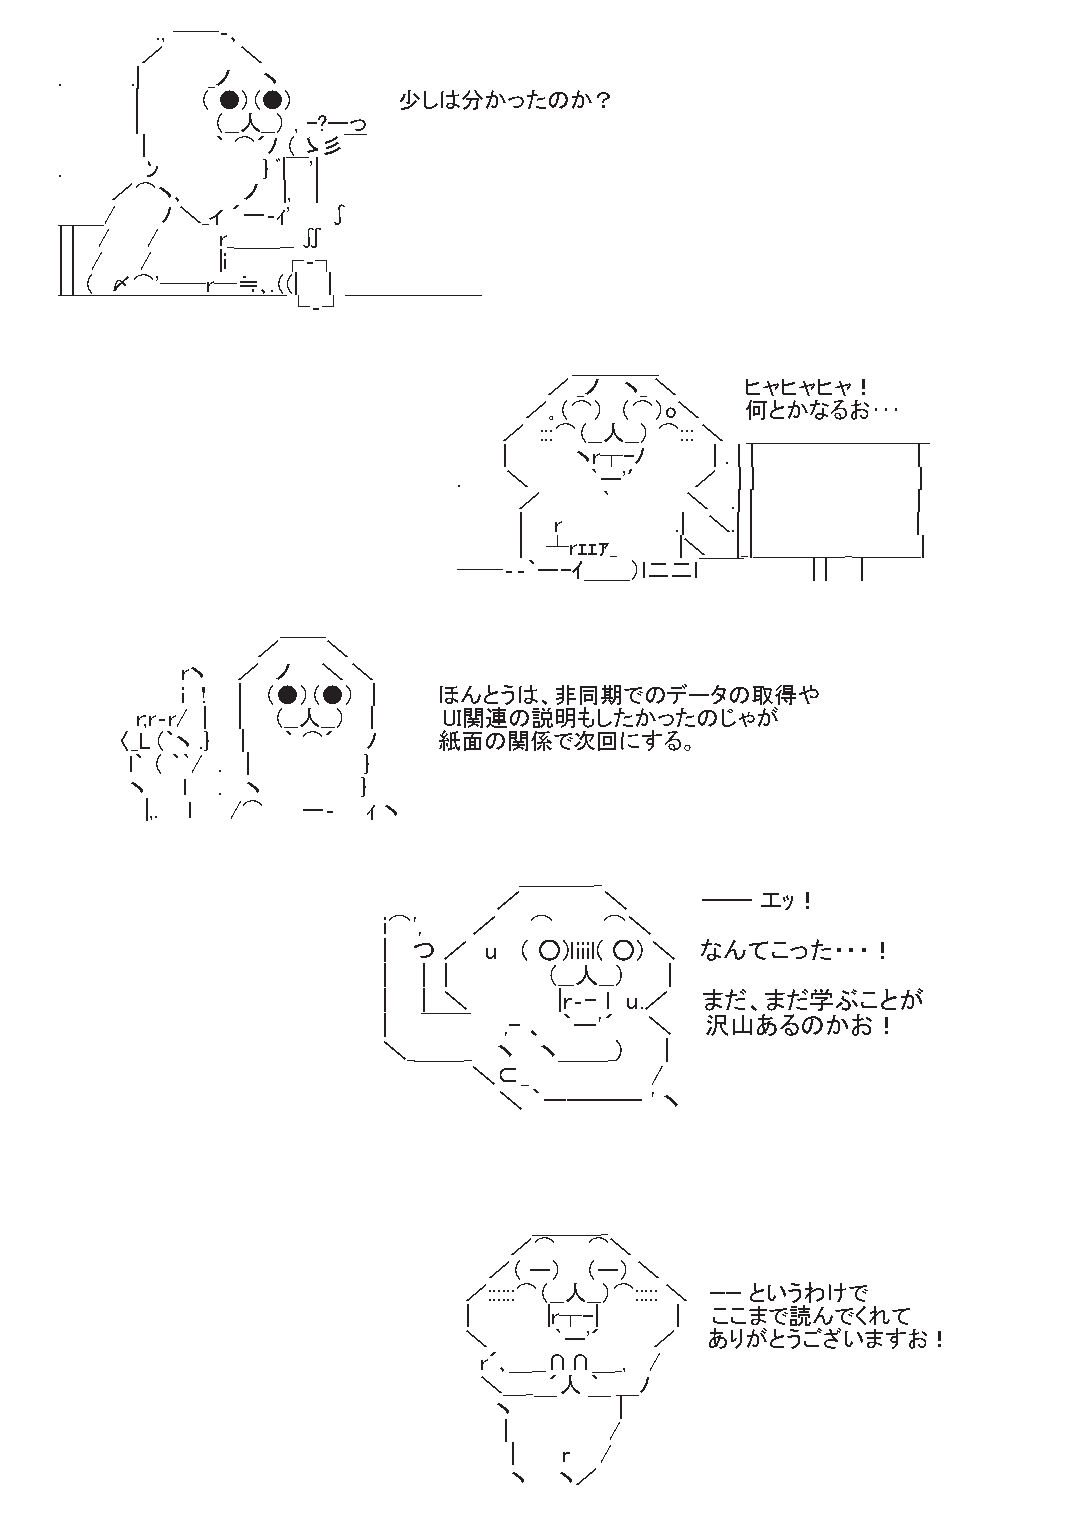
\includepdf[offset=2.3mm -2.3mm]{./images/cover_b5_back.pdf}
  \addtocounter{page}{-1}

\end{document}
